\section{\Grappa Overview}

Commodity hardware systems provide fast processors and high-bandwidth
interconnects but suffer when they encounter unpredictable data access
patterns. Maximizing throughput in such a situation depends upon proper
management of concurrency and communication. The \Grappa runtime
components handle thousands of concurrent accesses and batch them to
efficiently use the network. The imbalance between network bandwidth
and core-cycles for communication-intensive codes makes supporting
these functions in software an attractive design point. 
\Grappa specifically employs user-mode threading and networking for
low overhead because context switches and messages are very frequent.

As \Grappa depends on concurrency for performance, its programming
model focuses on enabling programmers to express large amounts of
concurrency. The overall goal is for the system to provide the
critical components for a well-performing implementation of an
irregular application, allowing the programmer to foremost focus on
expressing concurrency. While the programmer can initially be
productive in a shared memory environment and rely on the
underlying runtime components for reasonable performance, \Grappa
provides constructs for optimizing for locality and overlapping
communication.

\Grappa comprises three main software components, shown in Figure~\ref{fig:grappa}:

\begin{figure}[t]
\begin{center}
  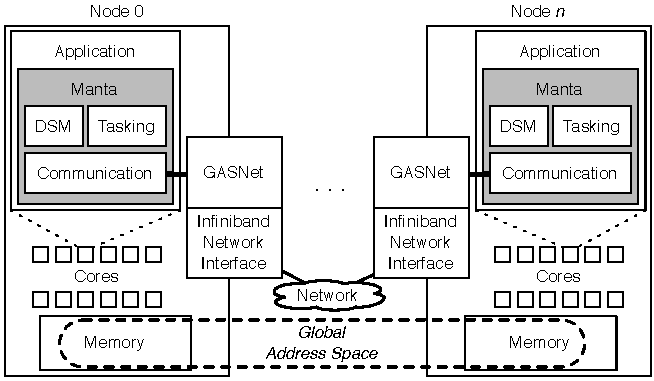
\includegraphics[width=0.95\columnwidth]{figs/system-overview}
\begin{minipage}{0.95\columnwidth}
  \caption{\label{fig:grappa} \Grappa system overview}
\end{minipage}
\vspace{-3ex}
\end{center}
\end{figure}

\begin{description}

\item [Tasking system.] The tasking system supports lightweight multithreading
to tolerate communication latency and global distributed work-stealing (i.e.,
tasks can be stolen from any node in the system), which provides automated
load balancing. The scheduler oversubscribes to have more worker threads than
required for latency tolerance. By keeping at least four workers per 
core ready to run at all times, the scheduler can prefetch a worker's state
into cache to reduce the chance of stalling on memory accesses during a
context switch.

\item[Communication layer.] The main goal of our communication layer is to
aggregate small messages into large ones.  This process is invisible to the application
programmer. Its interface is based on active messages~\cite{vonEicken92}.
Since aggregation and deaggregation of messages needs to be very efficient, we perform the process in parallel and carefully use lock-free synchronization
operations.
\TODO{Re-include the mention of GASNET,MPI spawning,and inifiniband
    somewhere but not in the overview intro}

\item[Distributed shared memory.] The DSM system provides fine-grain access to
data anywhere in the system, with delegated operation at the core of its design.
Every piece of global memory is owned by a particular core in the system, and all others may only access that memory by delegating their requests to the owning core.
It supports normal access operations such as
\emph{read\/} and \emph{write\/} as well as synchronizing operations such as
\emph{fetch-and-add\/}~\cite{fetchandadd}. Due to delegation, the memory model offered is similar to what underpins
C/C++~\cite{N2480,N2800}, so it is familiar to programmers. The DSM system
design relies on the lightweight tasking system and communication layer in
order to offer high aggregate random access bandwidth for accessing remote
data.

\end{description}
